\documentclass[12pt]{article}


\usepackage[dvips,letterpaper,margin=0.75in,bottom=0.5in]{geometry}
\usepackage{cite}
\usepackage{slashed}
\usepackage{graphicx}
\usepackage{amsmath}


\usepackage[american,fulldiode]{circuitikz}

\begin{document}
\ctikzset{bipoles/thickness=1}
\ctikzset{bipoles/length=.6cm}

\section{Introduction}

In this two-week long lab, which will require a long lab write-up, you
will build the data acquisition (DAQ) unit for a Geiger counter.  You
will compare the data you collect using your custom DAQ to compare
with the theoretical expectations for Poisson and Gaussian distributed
random variables.

\begin{figure}[htbp]
\begin{center}
{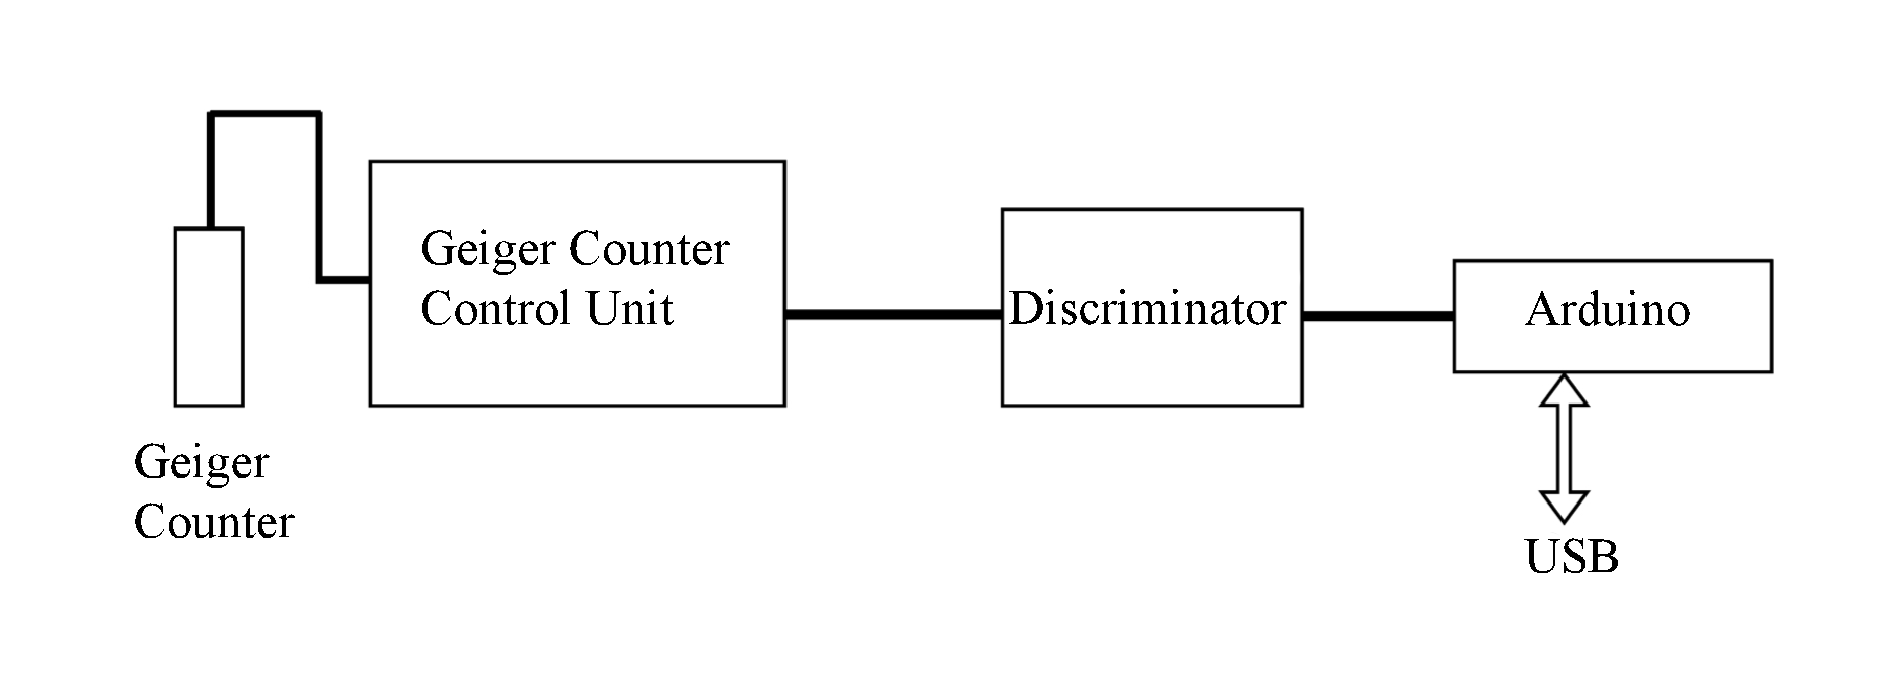
\includegraphics[width=0.75\textwidth]{figs/plan.pdf}}
\end{center}
\caption{\label{fig:plan} An overview of the lab setup.  The Geiger
  counter and control unit are provided.  You will build the
  discriminator stage and program an Arduino to complete the DAQ.}
\end{figure}

\begin{figure}[htbp]
\begin{center}
{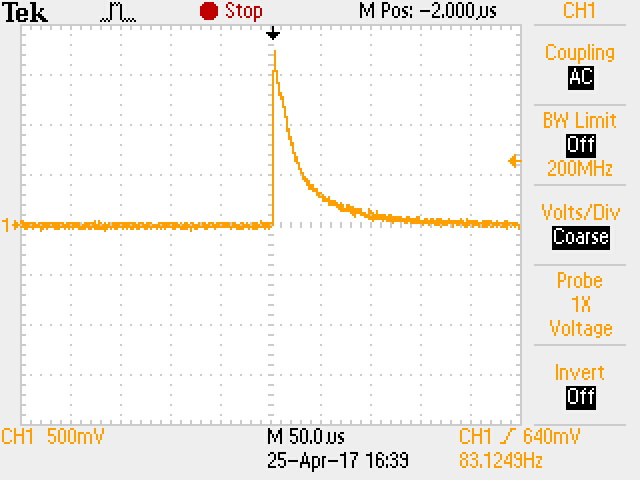
\includegraphics[width=0.55\textwidth]{figs/geiger_pulse.jpg}}
\end{center}
\caption{\label{fig:geigerpulse} Typical pulse from the Geiger counter}
\end{figure}

An overview of the lab setup is shown in Fig.~\ref{fig:plan}.  Once
properly setup, the Geiger counter will produce a pulse like the one
shown in Fig.~\ref{fig:geigerpulse} each time ionizing radiation
passes through the chamber.  The scope trace is AC-coupled, and
therefore does not show the 5 volt offset (called a pedestal) that is
present at the output.  The first stage of the discriminator removes
this pedestal with a high-pass filter.  The subsequent stages convert
these pulses above threshold into 5 volt digitized TTL pulses.  Once
connected to the Arduino, the DAQ unit receives a single TTL digital
pulse on an input pin for each incident ionizing particle.  The DAQ
simply counts these pulses during a fixed time interval and reports
the results over the serial connection.  You'll build the
discriminator, the DAQ, collect the data, analyze it using scientific
python, and report everything in a long writeup.

\section{Precautions}

\noindent
{\em Precautions with the Geiger counter:}
\begin{itemize}
\item Leave the cable from the Geiger counter controller to the Geiger counter in place {\em at all times}.  This carries voltages of approximately 1000 volts.  If you leave the cable in place, nothing can be inadvertently plugged in (including fingers!)
\item Leave the Geiger tube in its holder.  It has a thin front window which is easily broken.
\end{itemize}

\noindent
{\em Precautions with the radioactive source:}
\begin{itemize}
\item Don't touch the source.
\item Leave the source in the tray at all times.  The TA will provide the sources and handle moving them from place to place.
\item Radiation falls off as $1/r^2$.  So minimize your time near sources and maximize your distance from them.
\item Further information on radiation safety can be found in Melissinos and Napolitano.
\end{itemize}

\section{AC-coupled Schmitt Trigger}

The first stage of the DAQ is a Schmitt trigger discriminator based on the LM311 (See Fig.~\ref{fig:lm311}) that you will build yourself.  The LM311 is intended for TTL ($5~V$) logic and can be driven with a single-ended voltage all the way down to $5~\rm V$.  This makes it an ideal component to use with our $5~\rm V$ Arduino Uno.  We can power the LM311 from the Arduino $5~\rm V$ supply and send it's output directly to the Arduino.  There is no need to get out the bench-top DC supplies!

\begin{figure}[thbp]
\begin{center}
{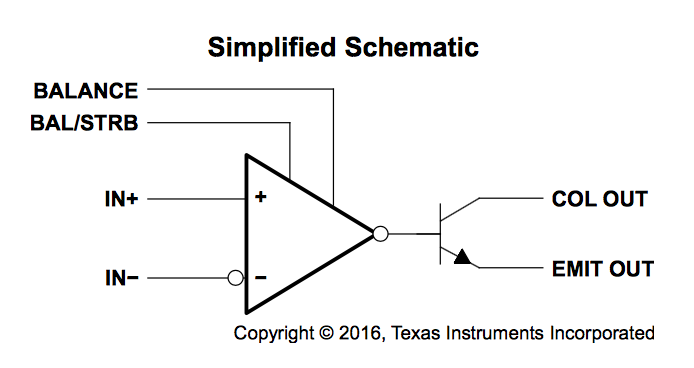
\includegraphics[height=0.2\textheight]{figs/LM311-scheme.png}}  \\
(a) \\ \vskip 1cm
\begin{tabular}{cc}
{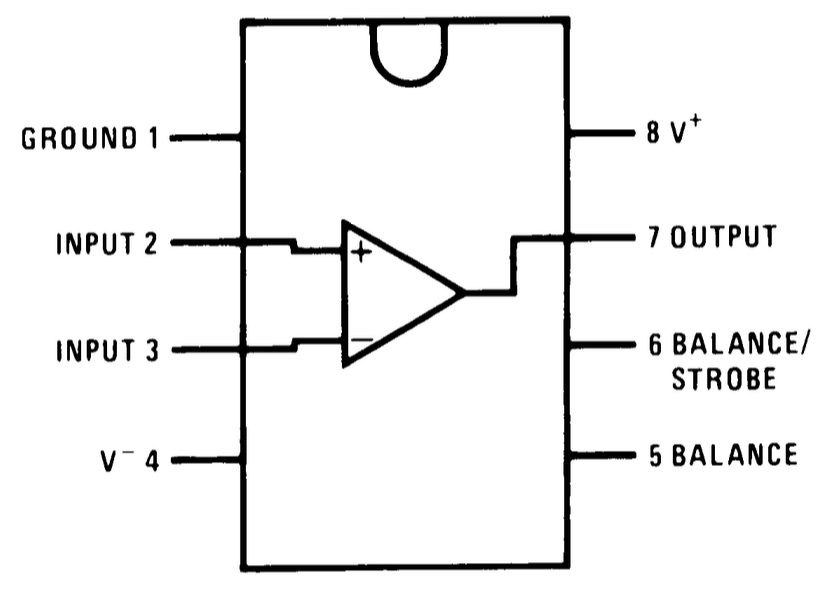
\includegraphics[height=0.2\textheight]{figs/LM311.png}} &
{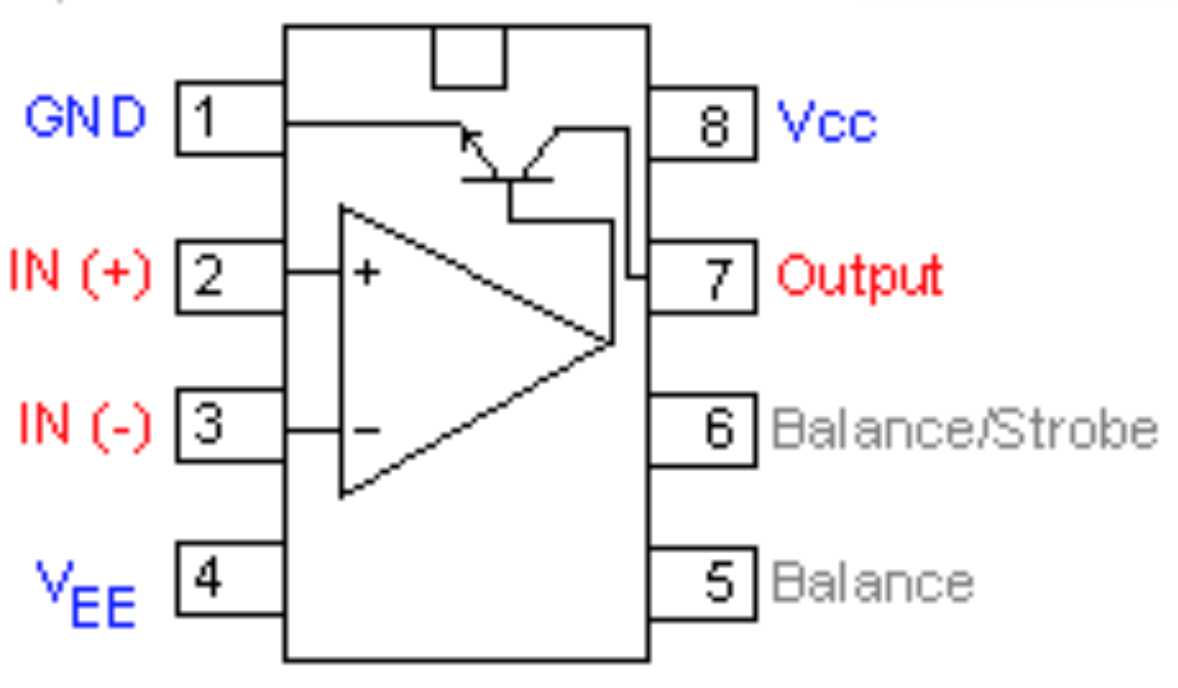
\includegraphics[height=0.2\textheight]{figs/LM311-trans.png}} \\
(b) & (c) \\
\end{tabular}
\caption{\label{fig:lm311} The LM311 (a) schematic from datasheet, and in 8-pin PDIP as (b) conventionally and somewhat deceptively shown, and (c) with the output transistor explicitly shown.  The version (b) is still slightly deceptive, as it leaves out the not operation between the op-amp and the transistor base.}
\end{center}
\end{figure}


The LM311 is an open-emitter open-collector comparator, that is, an op-amp driving the base of an NPN diode with both the collector and emitter available as outputs.   Typically the emitter of the output transistor is tied to ground and the collector output is therefore either grounded or high-impedance.  For this reason, a pull-up resistor is generally needed at the the collector output, so that the output is either $V_{\rm CC}$ or ground, depending on which of the two inputs is largest.

\begin{figure}[htbp]
\begin{center}
\begin{circuitikz}[line width=1pt]
\draw (0,0) node[op amp, yscale=-1](opamp){}  ++(2,0) node[not port](not){} ++(2,0) node[npn](npn){};
\draw (opamp.out) to[short] (not.in);
\draw (not.out) to[short] (npn.B);
\draw (npn.C) node[right]{$(7)$} to[short,-*] ++(0,0.5) coordinate(X) to[short,-o] ++(1.0,0) node[right]{$v_{\rm out}$} ;
\draw (X) to[R,l_=$R_4$,-*] ++(-5.5,0) coordinate(Y) |- (opamp.+); 
\draw (X) to[R,l_=$R_5$] ++(0.0,1.5) coordinate(X) to[short,-o] ++(0.5,0) node[right]{$V_{\rm CC}$} ; 
\draw (X) to[short,*-] ++(-6.0,0.0) to[R,l_=$R_2$] ++(0.0,-1.5) coordinate(X) to[short] (Y);
\draw (X) to[R,l_=$R_3$,*-] ++(0.0,-1.5) coordinate(Y);
\draw (npn.E) node[right]{$(1)$} to[short,-*] ++(0,-1.5) coordinate(X) node[ground, yscale=2.0]{};
\draw (X) to [short,-*] ++(-6.0,0) coordinate(X) to[short](Y);
\draw (opamp.-) node[below]{$(3)$} to[short,-*] ++(-2.0,0) coordinate(Y) to[R,l=$R_1$] ++(0.0,-1.5) |- (X);
\draw (opamp.+) node[above]{$(2)$};
\draw (Y) to[C,l=$C_1$,-o] ++(-1.5,0.0) node[left]{$v_{\rm in}$};
\draw (1.0,-0.75) node[below]{LM311};
\draw (5.5,-1.15) node[above]{$(4)$} node[ground,yscale=2.0]{};
\draw (6.5,-0.4) node[below]{$(8)$} to[short,-o] ++(0,0.5) node[right]{$V_{\rm CC}$};
\end{circuitikz} 
\caption{An AC-coupled inverting Schmitt trigger based on the LM311.  The LM311 IC provides both the operational amplifier and the transistor. The numbers in parenthesis are pin numbers.}
\label{fig:discrim}
\end{center}
\end{figure}

The discriminator circuit you will be building is shown in Fig.~\ref{fig:discrim}.  The input to the discriminator
is AC coupled by $R_1$ and $C_1$, which is needed to remove the pedestal (DC offset) present at the Geiger counter output.  This input is compared to a threshold predominantly set by the voltage divider $R_2$ and $R_3$.  When the input signal (at the {\em inverting} input) exceeds this threshold, the base of the transistor is driven high (note the NOT) and so the output is pulled to ground.  When the input signal is below the threshold, the base of the transistor is driven low, and the output is at $V_{\rm CC}$, due to pull-up resistor $R_{\rm 5}$.  The feedback resistor $R_4$ add hysteresis to the circuit, providing stability by pulling the threshold slightly higher once the output is high, and slightly lower once the output is low.

Build the circuit shown in Fig.~\ref{fig:filter} using $R_1=4.7~{\rm k\Omega}$, $C_1=10~{\rm nF}$,
$R_2=8.2~{\rm k\Omega}$, $R_3=1.1~{\rm k\Omega}$, $R_4=82~{\rm k\Omega}$, $R_5=1.1~{\rm k\Omega}$.  

\begin{figure}[htbp]
\begin{center}
{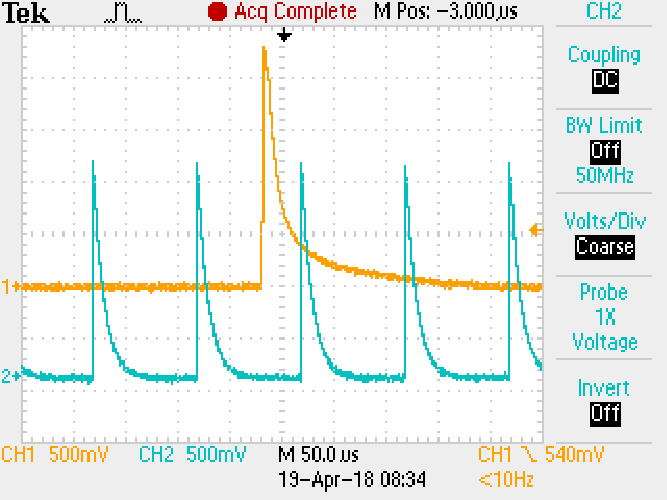
\includegraphics[width=0.55\textwidth]{figs/fake.pdf}}
\end{center}
\caption{\label{fig:fake} Side-by-side comparison of an actual Geiger output with the exponential decay function you will use to debug your data acquisition system.}
\end{figure}

For testing, you will need a reliable test signal that resembles the Geiger counter output.  Use your Tektronix AFG1022 function generator, and select the ``ExpDecay'' from Arb/Others/Built-in/Maths.
Set the frequency to $1~\rm kHz$ and the amplitude to $2~\rm V$ peak-to-peak.  A side-by-side comparison of the exponential decay function and actual output from the Geiger counter is shown in Fig.~\ref{fig:fake}.  Typical output from the discriminator is shown in Fig.~\ref{fig:typout}.  Once you circuit is working properly, it is amusing to remove the feedback resistor $R_4$ and observe the resulting instability, as shown in Fig.~\ref{fig:bounce}.

\begin{figure}[htbp]
\begin{center}
{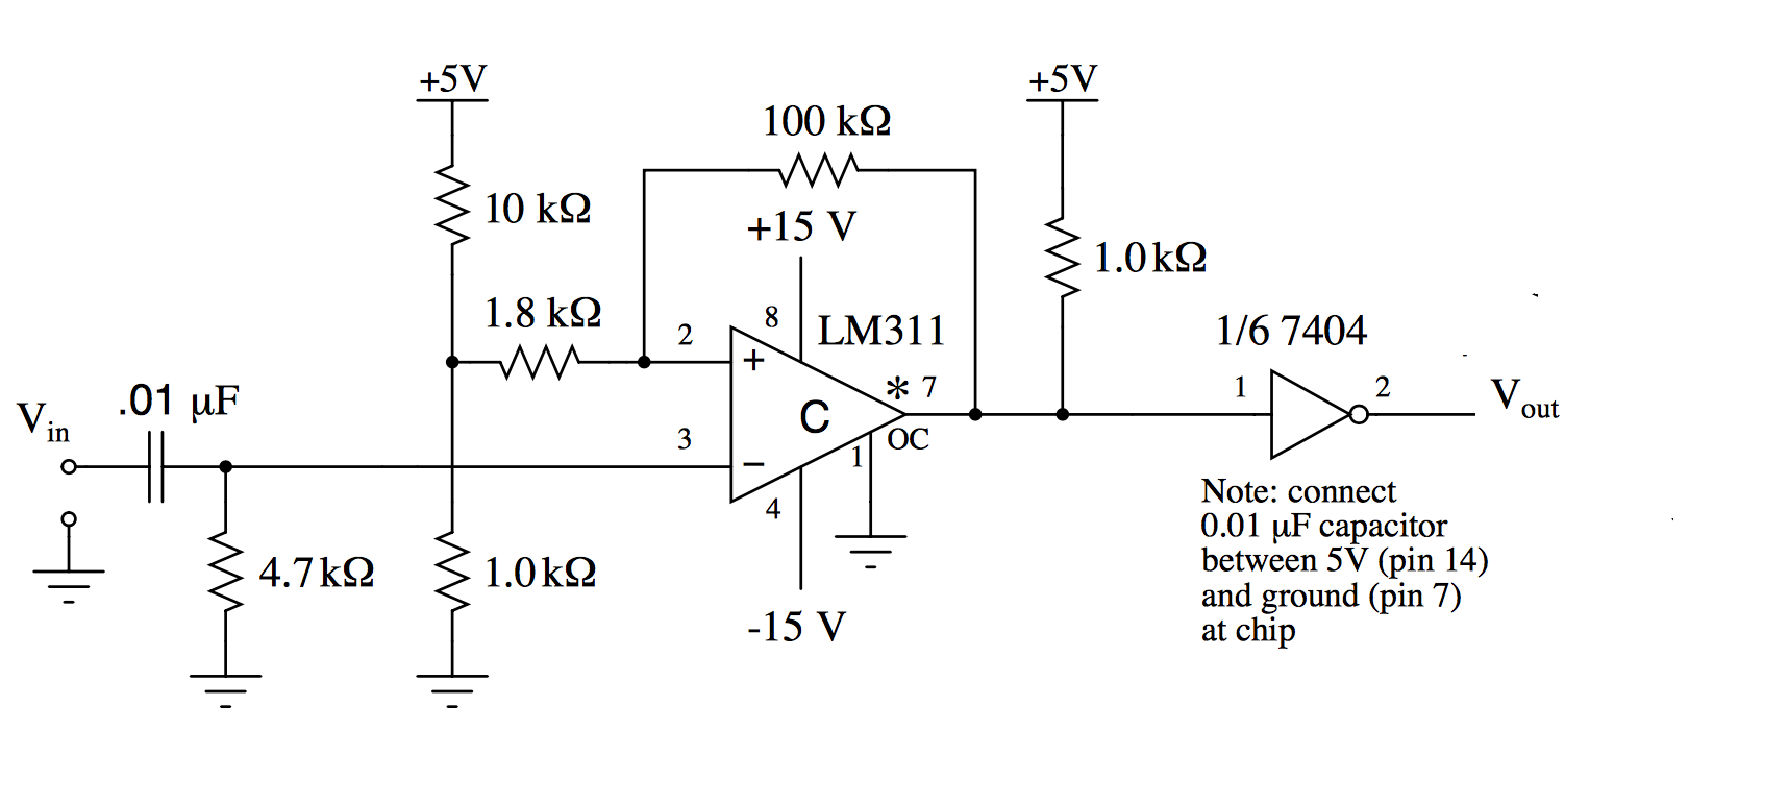
\includegraphics[width=0.55\textwidth]{figs/discrim.pdf}}
\end{center}
\caption{\label{fig:typout} Typical output $v_{\rm out}$ of the discriminator circuit (at pin 7 of the LM311) compared to the input $v_{\rm in}$ (at pin3 of the LM311).}
\end{figure}

\begin{figure}[thbp]
\begin{center}
\begin{tabular}{cc}
{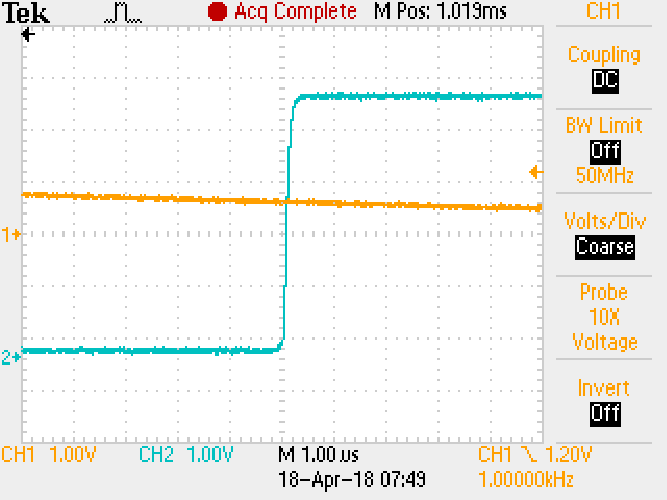
\includegraphics[height=0.25\textheight]{figs/schmitty.pdf}} &
{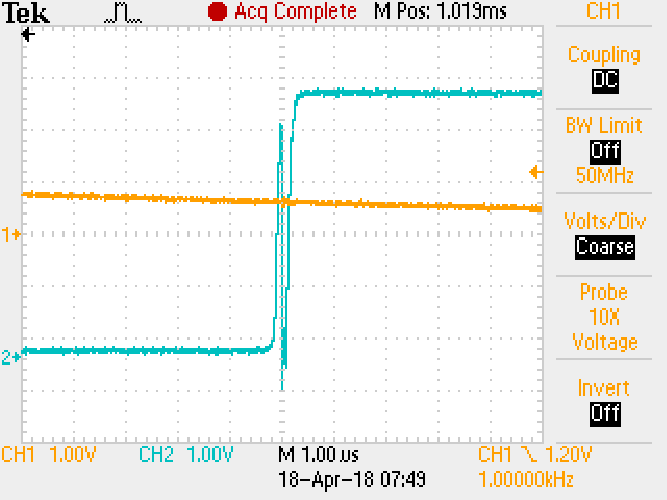
\includegraphics[height=0.25\textheight]{figs/bouncy.pdf}} \\
(a) & (b) \\
\end{tabular}
\caption{\label{fig:bounce} Single trace for the rising edge of the discriminator circuit (a) as designed, and (b) with feedback resistor $R_4$ removed from the circuit.  Without feedback, there is no hysteresis, and the output is bouncy.  Once you have your DAQ working, you can check what removing this resistor would do to the stability and accuracy of your rate measurement.  Spoiler alert:  you need it!}
\end{center}
\end{figure}


\section{Arduino Scalar}

The next step in your DAQ is Arduino scalar.  The scalar, or counter, will simply count the number of discriminator pulses that arrive during an adjustable time interval.  These sums, and the duration of the time interval, will be displayed on the serial interface for your to analyze offline.

The output of your discriminator circuit is easily handled by an Arduino microprocessor, as it has already been digitized at the $5~V$ logic level used by your Arduino Uno.  The digital pulses have a width of tens of microseconds, easily handled by an interrupt driven Arduino!

To get you started, an example sketch, ``Interrupts", is available on the course website:

\begin{verbatim}
const byte ledPin = LED_BUILTIN;
const byte interruptPin = 2;
volatile byte state = LOW;

void setup() {
  pinMode(ledPin, OUTPUT);
  pinMode(interruptPin, INPUT_PULLUP);
  attachInterrupt(digitalPinToInterrupt(interruptPin), blink, RISING);
}

void loop() {
  digitalWrite(ledPin, state);
}

void blink() {
  state = !state;
}
\end{verbatim}

This simple sketch sets up an interrupt service routine ({\tt blink}) to handle interrupts on the rising edge of transition on digital pin 2.  Every rising edge will cause the led to change state.  If you connect your discriminant output to the Arduino digital pin 2, and turn the frequency of the function generator down to $1 Hz$, you should observe the led to blink at 1 Hz.

Once you have this working, you should modify the blink interrupt service routine (suitably renamed!) to
\begin{itemize}
\item increment a count by one for every RISING (or FALLING) edge.
\end{itemize}
And modify the {\tt loop()} function to do the following every time it is called:
\begin{itemize}
\item measure the current time in microseconds, via {\tt micros()}.
\item set the counter to zero.
\item delay for a set time interval (e.g. 1 second:  {\tt delay(1000); }
\item save the counter value
\item measure the current time in microseconds.
\item output the duration and count for this loop over the serial interface.
\end{itemize}
Technically, you should warn the compiler that the {\tt count} global variable is effective by an ISR by using the volatile keyword, e.g.:
\begin{verbatim}
volatile int count = 0;
\end{verbatim}

\section{The Geiger Counter}

On the Geiger Controller, start with the HV set to zero at both the analog knob and the HV on-off switch.   Turn on the device and set the mode to``Test".  In this mode, the counter will be incremented at a fixed rate of 60 Hz.   While in this mode, play around with the ``Count", ``Reset", and ``Lab-Chron" analog timer reset dial until you understand how all of these features work.

Next check that you have a source in the second highest drawer of the Geiger Counter holder, asking the TA for help if this is not the case.  Switch the mode back to ``Use", which will now use the Geiger counter as input to the count.  With the HV still off, place the controller in ``Count" mode, and verify that the rate, with no HV, is zero.  Now, with the controller still in ``Count" mode, turn on the HV and turn the dial until you first see the counter incrementing.  Turn up the voltage to the next interval of 50 volts (e.g. if it first starts incrementing at 730 volts, set the dial to 750 volts).

Tabulate the number of counts in a 10 seconds interval, twice for each voltage level, in 50 volt steps from your starting voltage up to 1000 volts.  Do not exceed 1000 volts.  From the data, select the start of the plateau region, where increasing the voltage by 50 volts raises the rate by less than $10\%$.  With another measurement, confirm that the rate at this plateau is of order 100 Hz (this will vary from source to source).

Look at the ``SCOPE" output of the Geiger counter controller on your oscilloscope, with AC coupling, and verify that you see output pulses similar to those in Fig.~\ref{fig:geigerpulse}.

\section{Connect the DAQ}

Now connect the ``SCOPE" output of the Geiger counter controller to the input of your discriminator circuit.  Now check the output of your discriminator and verify that you have the expected TTL output pulse relative to the input geiger counter pulses, as in Fig.~\ref{fig:expected}.
\begin{figure}[htbp]
\begin{center}
{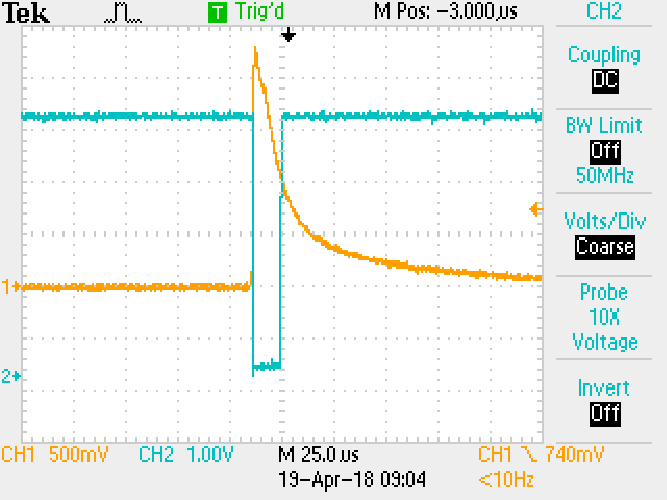
\includegraphics[width=0.55\textwidth]{figs/real.pdf}}
\end{center}
\caption{\label{fig:expected} Output of the discriminant from actual Geiger counter ouput.}
\end{figure}
With the shape of the digital input pulse verified, plug this in as input to your Arduino DAQ.  Verify that the rate you obtain with the Aruduino is within about $20\%$ of the rate you estimated with the timer and counter features.
 
\section{Collect and Analyze your Data}

Now you are ready to collect the data you will use for your analysis.  From your measured rate, estimate the $\tau$ and therefore $N_I$ needed to collect a mean $N_C$ of $1$,$5$, and $10$.  At each of these four values of $\tau$, collect the count for 100 individual runs.  Before leaving, verify that the mean value for each run is near the target mean value!  You could easily program your Arduino to take this average for you!  If time permits, also collect data from 1000 individual runs at each value of $\tau$.

\section{Long Report}

This lab report requires a long write-up.  Your TA will provide a Latex template for the report.  

To satisfy the writing requirements that this course satisfies, your report must be at least 15 pages long.  This is a terrible practice to put a minimum number of pages, as a hallmark of good writing is brevity and efficiency.  Therefore, we'll be enforcing this rule but will allow plots, figures, and appendices containing tables of your raw data, code listings (from both Arduino and Scientific python) to count toward this total.
Just put this long ``padding" material in the appendix, where it can be safely ignored by the TA, and concentrate on writing a concise accurate and complete report.

You should include an introduction describing the goals of the experiment and what you expect to observe, a discussion of your lab setup and procedure, plots and results from a toy Monte Carlo model for this experiment that you will develop with scientific python, actual results from your experiment, and a conclusion.

\end{document}
